\documentclass[a4paper]{report}

%====================== PACKAGES ======================

\usepackage[]{algorithm2e}

\usepackage{wrapfig}
\usepackage[french]{babel}
\usepackage[utf8x]{inputenc}
%pour gérer les positionnement d'images
\usepackage{float}
\usepackage{amsmath}
\usepackage{graphicx}
\usepackage[colorinlistoftodos]{todonotes}
\usepackage{url}
%pour les informations sur un document compilé en PDF et les liens externes / internes
\usepackage{hyperref}
%pour la mise en page des tableaux
\usepackage{array}
\usepackage{tabularx}
%pour utiliser \floatbarrier
%\usepackage{placeins}
%\usepackage{floatrow}
%espacement entre les lignes
\usepackage{setspace}
%modifier la mise en page de l'abstract
\usepackage{abstract}
\DeclareMathOperator{\Div}{div}
\DeclareMathOperator{\Rot}{rot}
%police et mise en page (marges) du document
\usepackage[T1]{fontenc}
\usepackage[top=3cm, bottom=2.8cm, left=2.5cm, right=2.5cm]{geometry}
%Pour les galerie d'images
\usepackage{subfig}
\usepackage{pgf, tikz}
\usepackage{amssymb}
\usepackage{pdfpages}
\usepackage{graphicx}

%====================== INFORMATION ET REGLES ======================

%rajouter les numérotation pour les \paragraphe et \subparagraphe
\setcounter{secnumdepth}{4}
\setcounter{tocdepth}{4}

\renewcommand\thesection{\arabic{section}}

\hypersetup{							% Information sur le document
pdfauthor = {Mario Viti,},			% Auteurs
pdftitle = {Compte Rendu TME -
			Sujet du Projet},			% Titre du document
pdfsubject = {Compte rendu TME},		% Sujet
pdfkeywords = {TME, BIMA, MatLab, ...},	% Mots-clefs
pdfstartview={FitH}}					% ajuste la page à la largueur de l'écran
%pdfcreator = {MikTeX},% Logiciel qui a crée le document
%pdfproducer = {}} % Société avec produit le logiciel

%======================== DEBUT DU DOCUMENT ========================

\begin{document}

%régler l'espacement entre les lignes
\newcommand{\HRule}{\rule{\linewidth}{0.6mm}}

%page de garde
\begin{titlepage}
\begin{center}

% Upper part of the page. The '~' is needed because only works if a paragraph has started.

\begin{figure}[h]
    \begin{minipage}[c]{.46\linewidth}
        \centering

\includegraphics[width=0.8\textwidth]{./logo_upmc_sorbonne.png}~\\[1cm]
  
    \end{minipage}
    \hfill%
    \begin{minipage}[c]{.46\linewidth}
        \centering

\includegraphics[width=0.6\textwidth]{./logo-sorbonne.png}~\\[1cm]

    \end{minipage}
\end{figure}

\textsc{\LARGE Université Pierre et Marie Curie}\\[2cm]

\textsc{\Large }\\[0.7cm]

\vspace{2cm}
% Title
\HRule \\[0.4cm]

{\huge \bfseries Master IMA: PIMA\\

\huge \bfseries  Thymio-2 with Raspberry Pi and camera: vision-based navigation using image tags\\
\vspace{1cm}
Project report
\\[0.4cm] }

\HRule \\[1.5cm]

% Author and supervisor
\begin{minipage}{0.4\textwidth}
\begin{flushleft} \large
\emph{}\\
Student: Mario \textsc{Viti}\\
mario.viti@etu.upmc.fr\\
Advisor: Nicolas \textsc{Bredeche}\\


\end{flushleft}
\end{minipage}
%\begin{minipage}{0.5\textwidth}
%\begin{flushright} \large
%\end{flushright}
%\end{minipage}

\vfill

% Bottom of the page
{\large \today}

\end{center}
\end{titlepage}

~
%ne pas numéroter cette page

%\input{./abstract.tex}

%\tableofcontents
%\thispagestyle{empty}
%\setcounter{page}{0}
%ne pas numéroter le sommaire

%\newpage

%espacement entre les lignes d'un tableau
\renewcommand{\arraystretch}{1.5}


%\begin{document}

%\maketitle

\section{Project presentation}

\subsection{Presentation}
Realization of an embedded image processing/vision system solution for Raspberry\footnote{\url{https://www.raspberrypi.org/documentation/}} powered Thymio robots.
Thymio-2 were originally designed at EPFL\footnote{\url{https://www.Thymio.org/fr:Thymio}} and mostly used for educational experiments. They're easy to program, not expensive and have been extended with a Raspberry PI 3 on-board camera and battery to create a standalone robot (Figure \ref{fig:thy}). To design and run robotics experiment an ad hoc framework has been developed.


\subsection{ThymioPYPI framework}
\textbf{ThymioPYPI}\footnote{\url{https://github.com/nekonaute/ThymioPYPI}} is a framework for programming a Thymio2 with a Raspberry PI in Python 2.X developed at ISIR Institut des Systèmes Intelligents
et de Robotique\footnote{\url{http://www.isir.upmc.fr/}}. 
Experiments constitute the specific behaviour desired for the robots.
ThymioPYPI provides a network infrastructure for shipping software to the Thymios and monitoring the distributed system.

\subsection{Requirements}
The main product of the PIMA project has been an extension module program to support experiments in which image processing and or computer vision tasks are involved, such as recognition of obstacles and other Thymios. This slave application must run transparently at a minimum frequency of service \textit{fos} of \textbf{$10 hz$}. This constraint must be assured in order to avoid making decisions and actions inconsistent with the sorrounding environment. In order to achieve this goal, choices of implementation need to take into account the treadoff between performances and precision. The requests for the system where to recognize a precise tag, estimate its distance and roation of relatively to the camera point of view.
Rotation estimation wasn't sufficiently satisfying so it will not be discussed and left as a next step for improvement. Each Thymio robot will be associated with a tag as shown in Figure \ref{fig:thy}.

\subsection{Hardware and software}
Raspberry Pi camera uses CSI port connection which can be accessed via custom API in python 2.X. This API provides efficient stream caputure via a VGA video port. Raspberry Pi avaliable at ISIR comes with a built from source 2.4 Opencv\cite{OpenCV} library which is an essetial tool for image processing.

\begin{figure}[H]
\centering
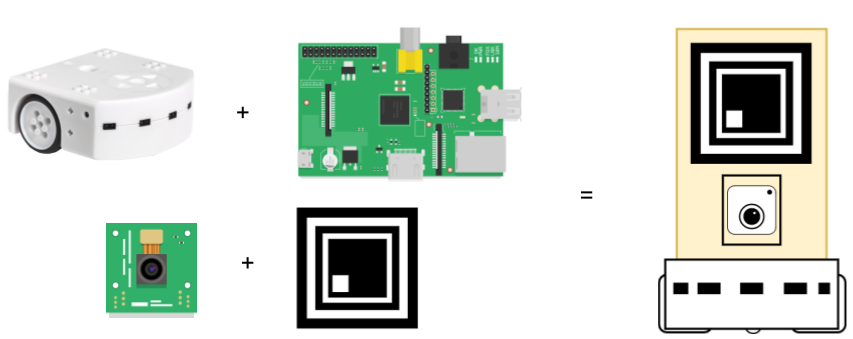
\includegraphics[width=0.9\textwidth]{standalone.png}
\caption{Thymio robot with Raspberry Pi, Camera and Tag.}
\label{fig:thy}
\end{figure}

\newpage 

\section{Tag detection in real time}

In this section a possible formalization of a realtime image processing application or detection task is proposed. 
A realtime image processing or detection task processes a stream of frames coming from a camera sensor and it can be defined as a service, slave or server application. As such, it must comply to provide the specified correct output within the other sole constraint of maximum time of service \textit{tos} or minimum frequency of service \textit{fos} imposed by the master or client. Thus it can be defined by the set \textit{\{outputs,tos\}}.

In the specific case of a \textit{tag detction} task, the correct outputs are: the contours of the tags present in the current frame, the identificators of each tag and the estimated distance from the camera.

When \textit{tos} constraints in time are narrow, to minimize \textit{tos} and maximize \textit{fos} a realtime processing task can be divided in 2 phases: a \textit{fine analysis} and a \textit{coarse analysis}.

\subsubsection{Fine analysis.}
A fine analysis consists of the best effort analysis of the current frame, this step is usually more computationally intensive than a coarse analysis.
For the proposed implmentation in tag detection \textbf{Algorithm \ref{alg:fine}} coincide with a fine analysis.

\subsubsection{Coarse analysis.}
The coarse analysis makes use of data acquired from the fine analysis, impling that fine analysis takes place before coarse analysis, for example as an hypothesis we assume that ideally little amount of change occours from frame to frame, therefore previous informations are still valid and coarse analysis uses fine analysis results to confirm or refuse the previously acquired beliefs and also tries to estimate current results as precisely as possible. For the proposed implmentation in tag detection \textbf{Algorithm \ref{alg:coarse}} coincide with the coarse analysis.\newline


\begin{algorithm}[H]
 \KwData{currentFrame}
 \KwResult{tagIDs, tagCountours, tagDistances }
 edgeImage = Canny(currentFrame)\;
 tagCountours = chekAreaRatio(edgeImage)\;
 tagImages = rectifyImage(currentFrame,tagCoutours)\;
 tagIDs = readID(tagImages)\;
 tagDistances = estimateDistances(tagCoutours)\;
 \caption{tagDetection}
 \label{alg:fine}
\end{algorithm}

\begin{algorithm}[H]
 \KwData{previousTagContours,previousFrame,currentFrame}
 \KwResult{tagCountours, tagDistances }
 tagContours = LKpyramid(previousFrame,currentFrame,previousTagContours)\;
 tagDistances = estimateDistances(tagCoutours)\;
 \caption{motionDetecion}
 \label{alg:coarse}
\end{algorithm}

\begin{algorithm}[H]
 frameCounter = 0\;
 frameBufferingLenght = 2\;
 Global running\;
 \While{running}{
 currentFrame = readFrameFromCamera()\;
 \eIf{frameCounter\%frameBufferLenght == 0}{
    tagIDs, tagCountours, tagDistances = tagDetection(currentFrame)\;
    }
    {
    tagCountours, tagDistances = motionDetecion(tagCountours,currentFrame,previousFrame)\;
    }
 frameCounter = (frameCounter+1)\%frameBufferLenght\;
 previousFrame = CurrentFrame\;
 \caption{postProcessing}
 }
 \label{alg:tgdt}
\end{algorithm}

\textbf{Algorithm \ref{alg:tgdt}} combines the two phases analysis and merges the results. The resulting $tos$ will be $ tos_{avg} = \frac{tos_{fine} + tos_{coarse}}{2} $ with $tos_{coarse}<tos_{fine}$ we'll achieve better performances on average.

\begin{wrapfigure}{r}{0.45\textwidth}
    \centering
    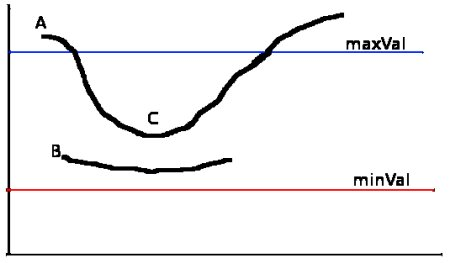
\includegraphics[width=0.45\textwidth]{hysteresis.jpg}
    \caption{Illustrating an example of a non connected edge thresholded by histeresis.}
    \label{fig:hist}
\end{wrapfigure}

\subsection{Edge detection}
For edge detection it has been adopted the popular solution of the Canny\cite{Canny} edge detection algorithm implementation in Opencv\footnote{\url{http://docs.opencv.org/2.4/doc/tutorials/imgproc/imgtrans/canny_detector/canny_detector.html?highlight=canny}}. This gradient based algorithm is suited to the task as it provides a luminance invariant simplification of the scene, meeting the requirement of tag detection in different lighting settings.
For this realtime application it has been used a varinat to the threshold values proposed by Canny in his paper to address the streaking issue resulting from the fluctuation in response of edges to the optimal operator.  For the \textit{histeresis filter} (Figure \ref{fig:hist})\footnote{Image source OpenCV documentation} min-max values are calculated starting from the mean $\hat{x}( 1 \pm \epsilon)$ luminance value sampled from the image. Thus sampling the whole image is costly, sample mean is computed by sampling different sub regions of the image in a \textit{Montecarlo} fashion. Connectivity is vital to the tag detection as tags are defined by enclosed sets of contours (more on the definition of the tag later in this document),this solution has proved to be more effective than fixed values in detecting tags in different light settings.

\subsection{Motion detection}
For motion detection another popular solution has been adopted: Lucas Kanade optical flow in its pyramidal variant also implemented in OpenCV\footnote{\url{http://docs.opencv.org/2.4/modules/video/doc/motion_analysis_and_object_tracking.html}}. \textit{"A matching process that must accommodate large displacements can be very expensive to compute. Simple intuition suggests that if large displacements can be computed using low resolution image information great savings in computation will be achieved. Higher resolution information can then be used to improve the accuracy of displacement estimation by incrementally estimating small displacemen"}\cite{LK}.
Although a hierarchical or multi resolution or pyramidal implementation of a motion field detector is independent of the field model, a pyramidal implementation of the LK optical flow alghotrithm can detect large quantities of motion as the constancy hypothesis of small amount of motion due to the linear approximation to the first term of Taylor series expansion still holds when images are subsampled and the \textit{brightness constancy constraint equation} is applyed to a small 5x5 pixels window. Furthermore as the purpose was to detect the shift of cornerlike features, this algorithm was best suited for the task.

\begin{figure}[H]
    \centering
    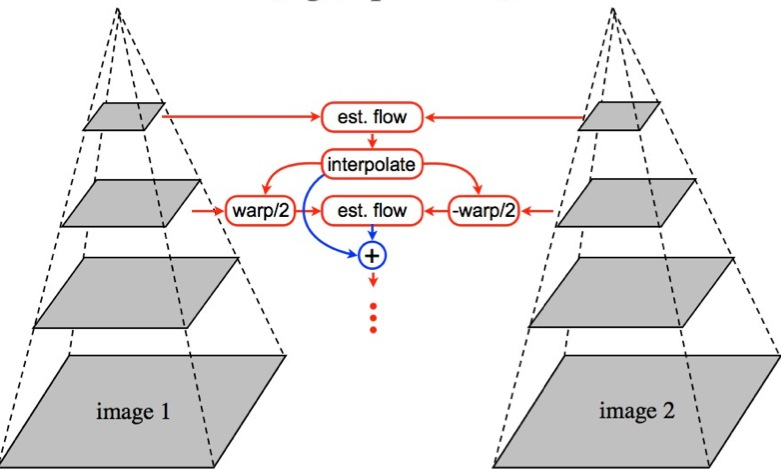
\includegraphics[width=0.6\textwidth]{lkp.jpg}
    \caption{Descriptive representation of a generic flow estimation pyramid.}
    \label{fig:lkp}
\end{figure}

\subsubsection{Treadoff}
As each level of the pyramid adds accuracy but also computations, the number of levels must be tuned accordingly in order to comply with the time of service constraints. For the presented solution a pyramid with 4 levels has been used with good results.

\section{Software development}

For the implementation of an image processing tasks a \textit{Python} package \textit{camera\_tools} has been developed to integrate the \textit{ThymioPYPI} framework.

\subsection{Design}

The software is designed as a \textbf{metaDetector}.

The metaDetector design abstraction is defined at multiple levels: it is a set of functions $\{$ \textit{preProcessing},\textit{postProcessing} $\}$ with the output of the \textit{preProcessing} is piped to the \textit{postProcessing} function as shown in \textbf{Algorithm \ref{alg:meta}}.
Furthermore it is an \textbf{Interface} for image processing implemented as \textbf{Class}, tag detection is realized by \textit{implementing} a \textit{metaDetector}. The nature of this division, the details of the preProcessing and postProcessing will be discussed further in the next section.\newline

\begin{algorithm}[H]
 \KwData{frame}
 \KwResult{postProcessingOutput}
 preProcessingOutput = preProcessing(frame)\;
 postProcessingOutput = postProcessing(preProcessingOutput)\;
 \caption{metaDetector}
 \label{alg:meta}
\end{algorithm}

For a more detailed description on the usage of the software it has been released the \textit{ThymioPYPI manual.}\footnote{\url{https://github.com/nekonaute/ThymioPYPI/blob/master/Robocologie_manual.odt}}. The most important modules of the package are:\newline

\fbox{\parbox{\textwidth}{\textbf{camera\_tools} package:\newline

    \begin{itemize}
    \item CameraController: handles RaspberryPi camera module PiCamera.\newline
    
    
    \item ImageProcessor: holds the CameraController and handles the buffer in which pixels are stored by applying preProcessing and postProcessing to it.\newline
    
        \subitem Detector: exposes the ImageProcessor capabilities by defining the metaDetector Interface.\newline
    
    \item TagDetector: implements the metaDetector interface.\newline
    \item image\_utils : collection of functions for image processing.\newline
    \item tag\_recognition : collection of functions for tag detection.\newline
    \end{itemize}

}}

\newpage 

\subsubsection{Realtime image processing}

The Raspberry Pi 3 model b is equipped with a \textit{1.2 GHz 64-bit quad-core ARM Cortex-A53} which allows different threads to execute on different cores.
A realtime application can exploit multithreading by definig a set of independet tasks. We'll define 3 types of independent tasks in our application.

\begin{enumerate}
    \item \textbf{capture}: this task is mostly camera bound and it involves capturing an image and converting it to readable byte format.
    \item \textbf{preProcessing}: in the previous section this was described as one part of the meta algorithm for image processing, it refers to any task that involves "non heavy" (linear in the sole image size) computation on images i.e. RGB to HSV conversion.
    \item \textbf{postProcessing}: in the previous section this was described as one part of the meta algorithm for image processing, it refers to any task that involves "heavy" (non linear in the image size) computation on images i.e. EdgeDetection involving convolution.
\end{enumerate}

This set of tasks defines a general realtime application running on a on board solution with or wihtout GPU support to maximize throughput.

Figure \ref{fig:lfcy} shows how the 3 different tasks need to be secured by locking critical session on shared buffer among threads. \textit{PreProcessing} function computional requirement is a suggestion as it's applyed to a shared buffer, sharing buffers limits memory usage but serializes computation. As an hypothesis keeping linear computation to the \textit{PreProcessing} step will ensure a capture request returning after \textit{PreProcessing} ended and a copy of the buffer is kept for \textit{postProcessing}.

\begin{figure}[H]
    \centering
    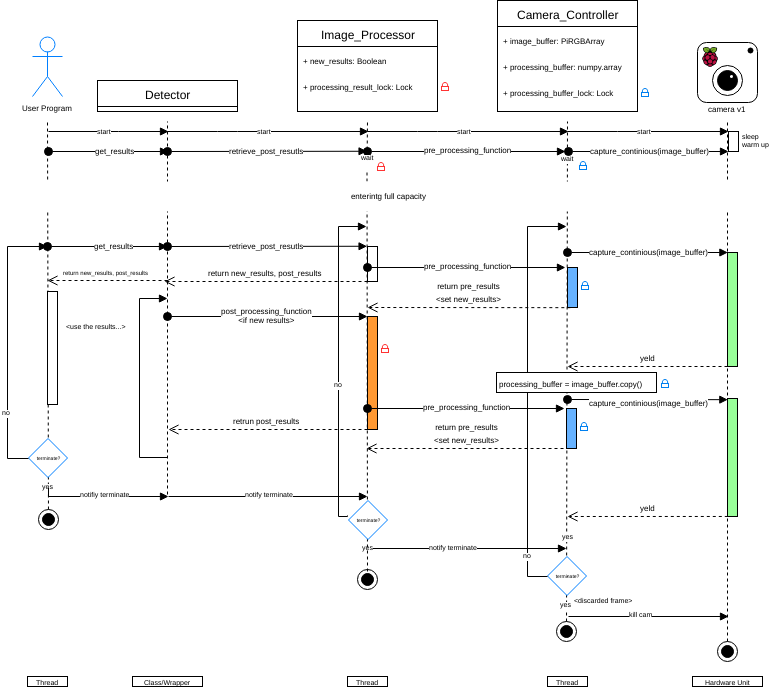
\includegraphics[width=0.9\textwidth]{Detector.png}
    \caption{lifecycle of a image processing realtime application.}
    \label{fig:lfcy}
\end{figure}


%\NOTA: Nuova pagina, serve per l'immagine wrapped sennò rimane mezza fuori nel fondo della pagina.
\newpage 

\section{Tags}

\subsection{Encoding}

\begin{wrapfigure}{r}{0.25\textwidth}
    \centering
    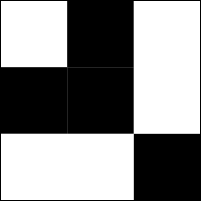
\includegraphics[width=0.25\textwidth]{reader.png}
    \caption{an example of a 3x3 bits encoded tag.}
\end{wrapfigure}

An encoded tag is modeled as a discreete bi-dimensional serie
$ e(x,y) = \sum_{i,j}^{n,m} a_{i,j} h(x-iS_{b},y-jS_{b}), n,m \in \mathbb{N}$ with $h(x,y) = Arect_{S_b}(x-S_b/2,y-S_b/2)$ and $T_b$ the \textit{space per bit} and $a_{i,j} \in \{ -1,1 \}$, the wave shape $h(x,y)$ and the simbol $a_{i,j}$ will encode the information in binary format. For better precision $m-ary$ encoding are better avoided because of the high noise in the communication channel.

The noise in the communication channel is modeled as an additive white gaussian noise or \textbf{AWGN} with constant dsp equal to $N_0$. In a one dimensional encoding while in presence of this noise applied to a signal just described the signal to noise ratio \textbf{SNR}  of an SLI filter or receptor $g_r(t)$ is maximixed by applying the \textit{Cauchy-Schwarz} inequality.

$$ SNR = \frac{\int_{-\infty}^{+\infty}g_r(t)h(t_0-t) dt}{\sqrt{N_0\int_{-\infty}^{+\infty}g_r(t)^2 dt}} \leq \frac{\sqrt{\int_{-\infty}^{+\infty}h(t_0-t)^2 dt}}{\sqrt{N_0}}$$

From which it is derived the analitical form of the optimal adaptive filter $g_r(t) \propto h(t_0 - t)$, this can be applied to the 2D case without loss of generality $gr(x,y) \propto h(x,y)$. 

\subsection{Reading}

\begin{wrapfigure}{l}{0.45\textwidth}
    \centering
    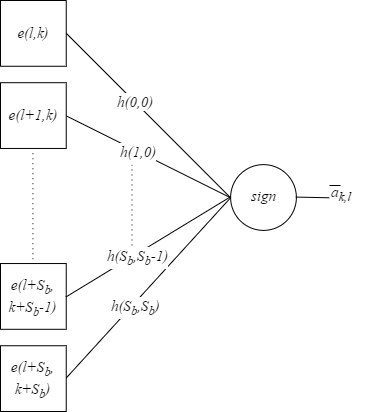
\includegraphics[width=0.4\textwidth]{reader_perce.png}
    \caption{perceptron reading one bit.}
\end{wrapfigure}

The sequence of symbols received $\hat{a}_{k,l}$ is the result of the sampling of the signal processed by the adaptive filter which consists of a meaningful term, or simply signal and a noise term. By means of the adaptive filter the signal term will be greater than the noise term, ideally.

$$\hat{a}_{l,k} = sign((h * h)(S_b/2,S_b/2)a_{l,k} + (n*h)(l,k))$$

with $n(x,y)$ being the \textbf{AWGN}  random signal and $(h * h)(T_b/2,T_b/2)a_{l,k} > (n*h)(l,k)$ respectively the meaningful and noise term. 

The discreete version of $(h * h)(T_b/2,T_b/2)a_{l,k}$ is a dot product $\sum_{i,j}^{S_b,S_b} Arect_{S_b}(i-S_b/2,j-S_b/2)e(l+i,k+j)$.

The computation involved in this "decisional process" is exactly the same that occours when using a \textit{perceptron}. In this case however the \textit{weitghts} for the linear classification ar not learned but computed anallitically, as in theory this is the optimal filter, a perceptron will tend to this solution.

%\NOTA: Fino a qua abbiamo una pagina perfetta quindi richiedo una nuova pagina per mantenere il layout fisso.
\newpage

\subsection{Perspective invariant feature detection}
\begin{figure}[H]
    \centering
    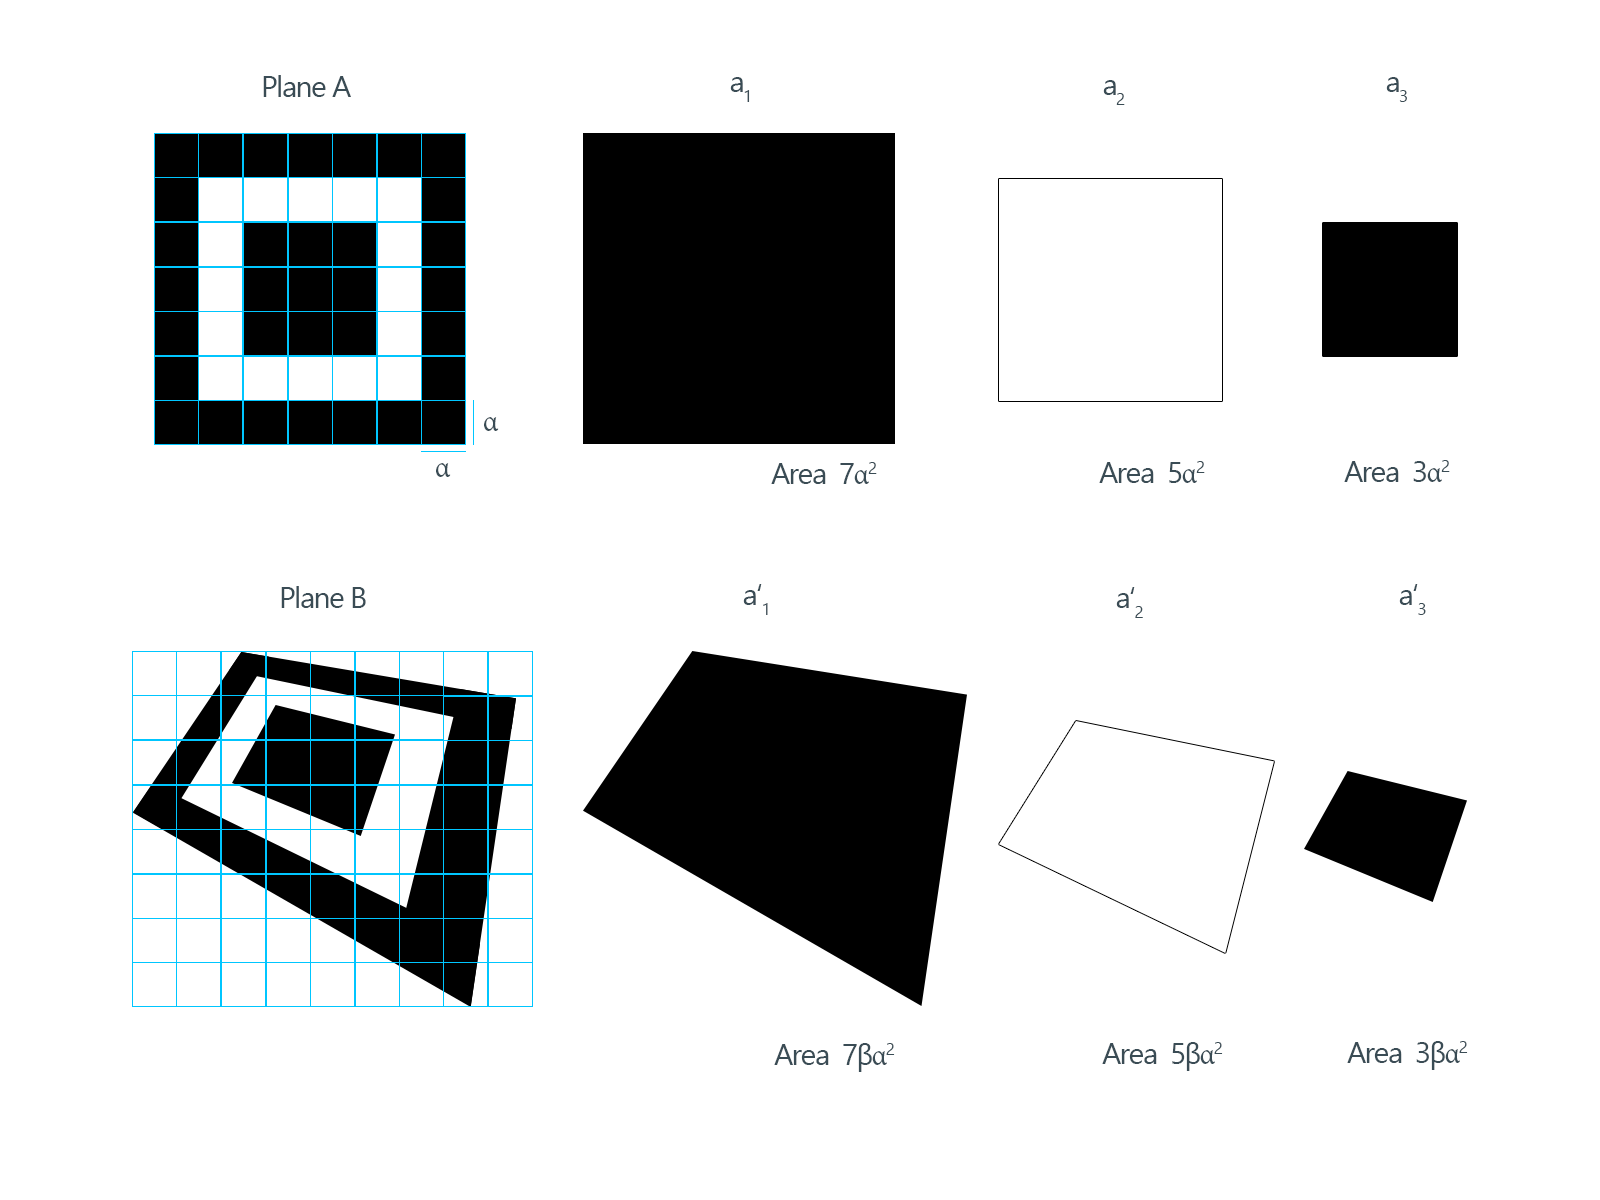
\includegraphics[scale=0.2]{area_ratio.png}
    \caption{area ratios for example tag with perspective transformation.}
\end{figure}
The first step in tag detection is to extract perspective covariant descriptors that minimize the complexity of the scene from which compute perspective invariant descriptors.
From a pair of two closed edges present in the image we can compute area ratios, closed edges represent the covariant descriptos from which a one dimensional feature is then extracted. This procedure can be used to identify a tag with a known area ratio within closed edges present in the tag itself, this technique has been first used in a very popular techonlogy: the QR code\cite{QR}.

The next phase involves the apriori knowledge of the shape of the tag.
Once the tag countour is identified in the frame, the warp or \textit{perspective transform matrix} can be estimated and inverted, by applying the inverse prespective transformation to the pixels within the detected contour ROI we obtain a rectified image that can be read as described previously.

\subsection{Tag description}

\begin{wrapfigure}{l}{0.45\textwidth}
    \centering
    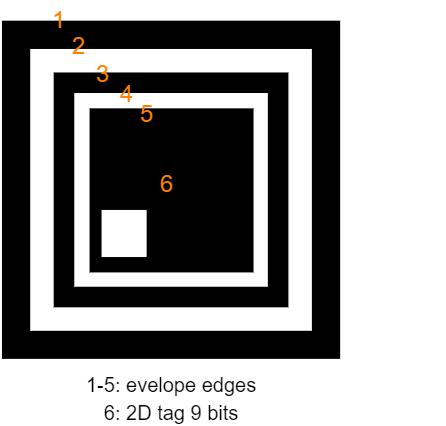
\includegraphics[scale=0.35]{tag_pro.png}
    \caption{custom Thymio Tags.}
    \label{fig:tagp}
\end{wrapfigure}

A custom tag has been developed for the Thymio robots as seen in Figure\ref{fig:thy}.

The ID number encoded information is embedded into several enclosed edges to ensure robustness to false positives.

In Figure \ref{fig:tagp} it is shown the hierarchical structure of edges , starting from the outermost to the innermost there are 3 generation of edges. For each edge $i$ a predecessor is the edge numbered with a number $j$ and $i<j$, between a father and a child the area ratio is know and it is used for a more roboust detection. The innermost square contains the information or tag ID encoded as described previously. The IDs are encoded into 9 bits yelding 512 possible configuration allthough two among these are better avoided (0 and 511).\newline \newline

\newpage 

\section{Results}

The tag detection system met the requirements of a minimum $fos \geq 10hz$ and reached a maximum of $12 hz$ this performences however are achieved in optimal settings, however problem arose wile testing and will be discussed in this section and the next.

\subsection{Tracking evaluation}

\begin{wrapfigure}{l}{0.6\textwidth}
    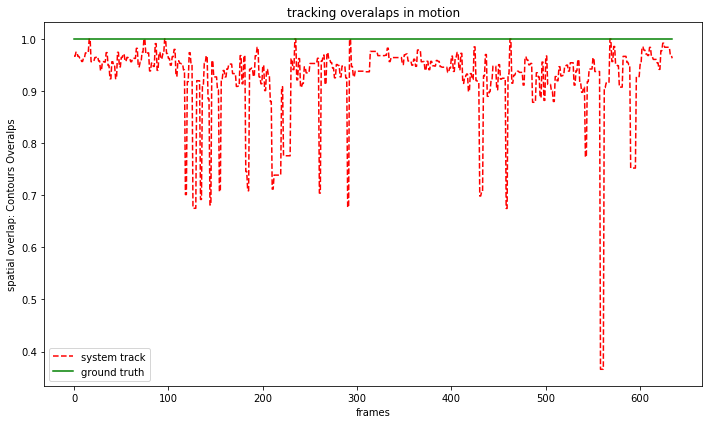
\includegraphics[width=0.6\textwidth]{rat1.png}
    \caption{different experimental settings.}
    \label{fig:ovlp1}
    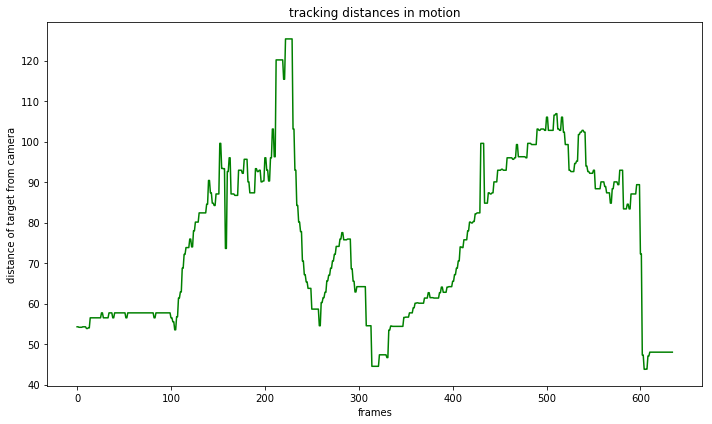
\includegraphics[width=0.6\textwidth]{rat2.png}
    \caption{different experimental settings.}
    \label{fig:ovlp2}
    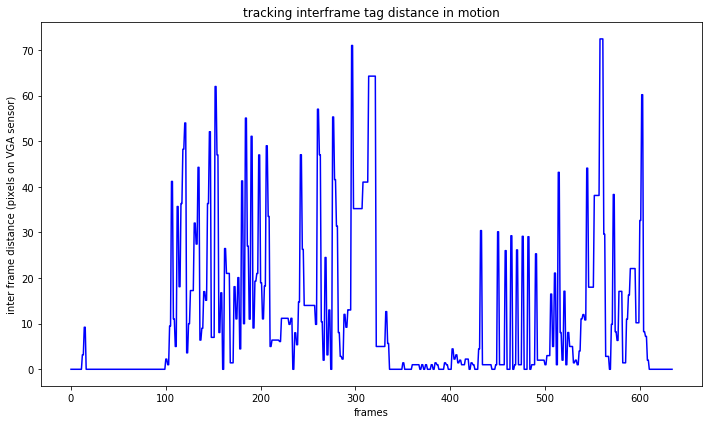
\includegraphics[width=0.6\textwidth]{rat3.png}
    \caption{different experimental settings.}
    \label{fig:ovlp3}
\end{wrapfigure}

This tag detection application can be evaluated as a \textbf{tracking system} as desrcibed in\cite{Performance}. We will use \cite{Performance} as a guideline for metrics and performance estimation practices as these has been used on other popular tracking systems.
The method description follows: \textit{"First we will define the concepts of spatial and temporal overlap between tracks, which are required to quantify the level of matching between Ground Truth (GT)  tracks and System (ST) tracks, both in space and time. The spatial overlap is defined as the overlapping level $A(GTi,  STi)$ between $GTi$ and $STi$ tracks in a specific frame $k$:"} \cite{Performance} $$ A(GTik,  STik) = \frac{Area( GTik \cap STik}{Area( GTik \cup STik} $$

In order to evaulate the performances an experiment has been set up in the arena with Thymio robots. A robot moved in front of the camera randomly, the tracking is executed once by using the \textit{fine analysis} on each frame (GT), subsequently the tracking is done by intervealing \textit{fine analysis} and \textit{coarse analysis}(ST) based on motion estimation, cotours overlaps are computed for each frame (Figure \ref{fig:ovlp1}). For each frame, distance from the camera (Figure \ref{fig:ovlp2}) and interframe distance (Figure \ref{fig:ovlp3})  are registered in order to correlate how distance from the camera and velocity affects the tracking system.

\textbf{False alarm track (FAT) of False Positive (FP):}

\textit{"Although  it  is easy  for  human  operators  to  realise what  is  a  false  alarm  track  (event)  even  in  complex situation,  it  is  hard for  an automated system to  do  so. Here, we give a practical definition of false alarm track"}\cite{Performance}. $$FAT=\frac{\sum_{k=0}^n A(GTik,  STik)}{n} < thr$$, $n=$ \# frames, $thr = 0.6$.\newline\newline

\textbf{Track matching error (TME):}

\textit{"This metric measures the positional  error  of  system tracks.
TME is the average distance error between a system track  and  the  GT  track.  The  smaller  the  TME,  the better the accuracy of the system track will be."}\cite{Performance}
In this application the distance is normalized with the maximal distance possible as the diagonal of the VGA window: $$TME=\frac{\sum_{k=0}^n Dist(GTik,STjk)}{n (VGA_d)} $$
\textit{"where  Dist()  is  the  Euclidean  distance  between  the centroids of GT and the system track: TMED is  the standard  deviation  of  distance  errors"}\cite{Performance}
In Figure \ref{fig:track} two tracks are overalapped as they appear on screen, specifically only the center of the contour is registered.

\begin{itemize}
    \item FAT: 0.005
    \item TME: 0.02
    \item TMED : 0.01
\end{itemize}

\begin{figure}[H]
    \centering
    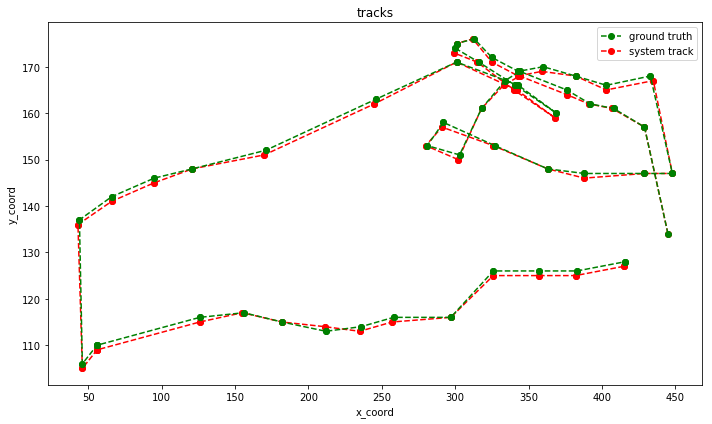
\includegraphics[width=1.0\textwidth]{tracks.png}
    \caption{different experimental settings.}
    \label{fig:track}
\end{figure}

\subsection{Experiments}

\subsubsection{Validation}

\begin{figure}[H]
    \centering
    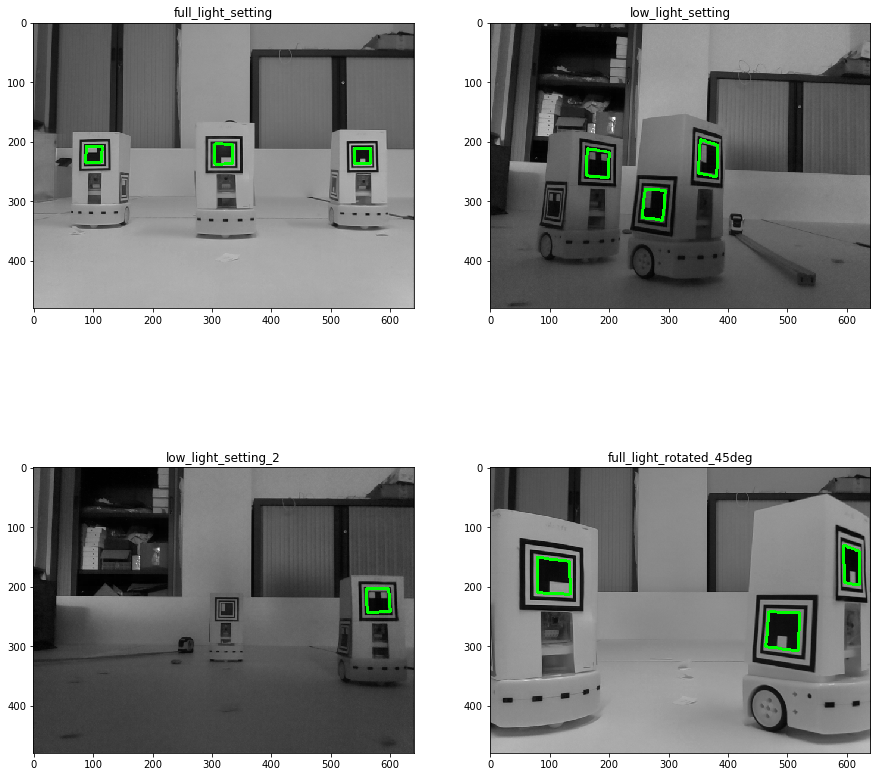
\includegraphics[width=1.0\textwidth]{fulll.png}
    \caption{different experimental settings.}
    \label{fig:sett}
\end{figure}

In order to evaulate the performances an experiment has been set up in an arena with Thymio robots. Each robot was positioned in a precise location and shown to the camera in order to cover all the visible area. This experiment is repeated in two different settings: a full light setting with homogeneus light coming from artificial lamps and a low light settings with noisy background, non homogeneus light and a gradient like soft shadow overlaying the scene. It is one last time repeated by changing the rotation with respecto ro the camera of 45° with mixed light settings.

In order to measure the performance it has been defined a per second \textit{frequency of detecion} as $\frac{hit_t}{max_t(hit_t)} $ where a $hit$ occours when tag $t$ is detected a number $hit_t$ of times per second and ${max_t(hit_t)}=fos$.

\textbf{Caveat}
These results are contingent to the setting: the size of the tag and the definition of the sensor influence the results as performance are in funtion of the area in pixels of the tag on the sensor which is a function of the tag real dimensions and the camera definition.

\fbox{\parbox{\textwidth}{Settings:
\begin{itemize}
    \item tag innermost side size: 4cm
    \item sensor definition: VGA (640,480)
\end{itemize}
}}

\begin{figure}[H]
    \centering
    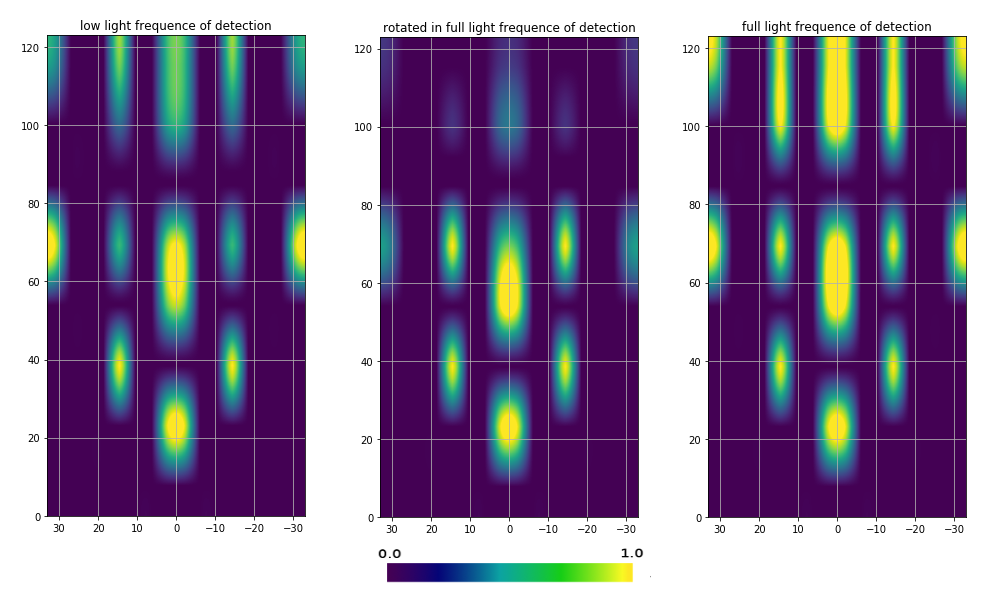
\includegraphics[width=1.0\textwidth]{heat.png}
    \caption{frequencies of detecion against positions (in cm).}
    \label{fig:freq_hit}
\end{figure}

Distance estimation has been evaluated against real distance from the camera.
In presence of low light and noise it's noticeable an higher variance in the error. Also it seems that a systematic bias is present in distance estimation when distance augments, this is probably due to the sampling of a continuos shape on a discrete grid which makes the apparent size different from the real size and introduces aliasing.

\begin{figure}[H]
    \centering
    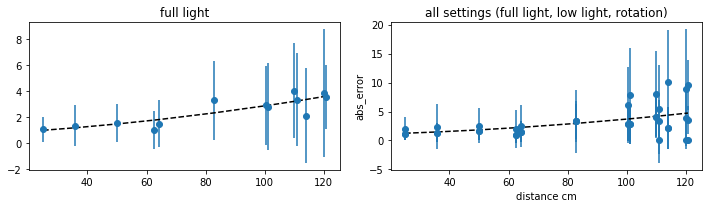
\includegraphics[width=1.0\textwidth]{distance.png}
    \caption{absolute error of real and estimated distance againts real distance, bars indicates variance in the absolute error.}
    \label{fig:dist}
\end{figure}

\subsubsection{Navigating the environment with image tags}

After validation a simple experiment has been designed to test the tag detection software. These experiment were designed to prove how the tag detection improves the behaviour of the robot and its interaction with its sorroundings. The experiment were designed with incremental difficulty for the robots.

\textbf{Experiment 1: Followers} There are 2 Thymio robots acting in this experiment (Figure \ref{fig:folltg} left) each robot moves foreward and follow the tag when in view. \textit{Thymio1} tries to reach a target, \textit{Thymio2} just follows the first.

\textbf{Experiment 2: Avoiders} (Figure \ref{fig:folltg} center) This experiment is opposite or dual to experiment 1, robots behaviour is to avoid any tag if seen.

\textbf{Experiment 3: Avoiders and target seeker} (Figure \ref{fig:folltg} right) this experiment increases difficulty for the Thymio robots. There are still 2 actors in this setting but the behaviour changes: each robot must avoid each other and try to reach the target (which is identified by a different id).

\begin{figure}[H]
    \centering
    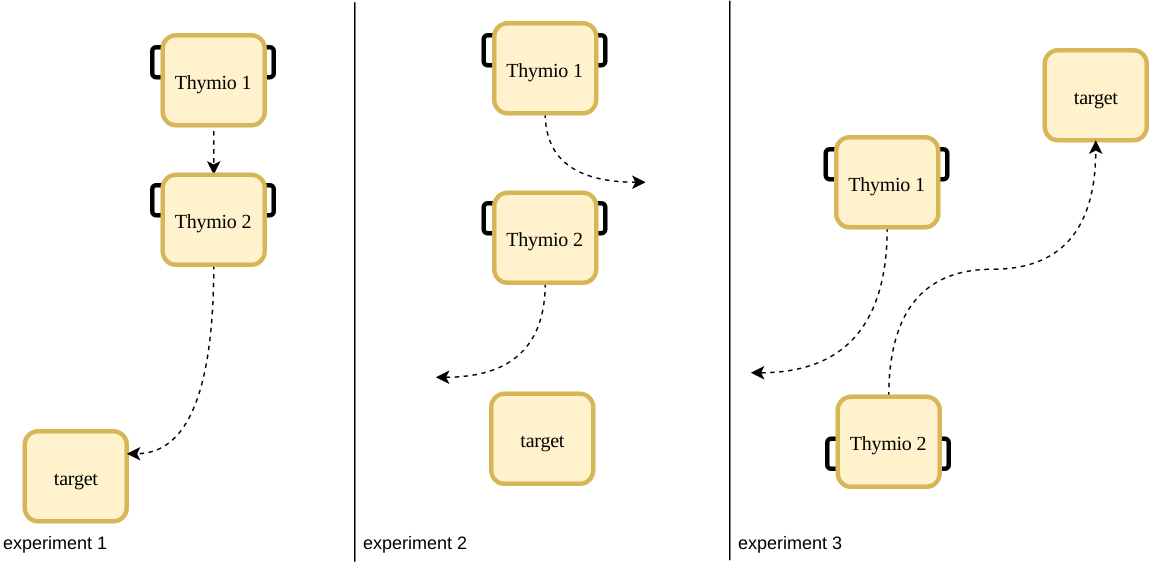
\includegraphics[width=1.0\textwidth]{experiment.png}
    \caption{Experiment follow tag setting 1 and 2.}
    \label{fig:folltg}
\end{figure}

\begin{wrapfigure}{l}{0.5\textwidth}
    \centering
    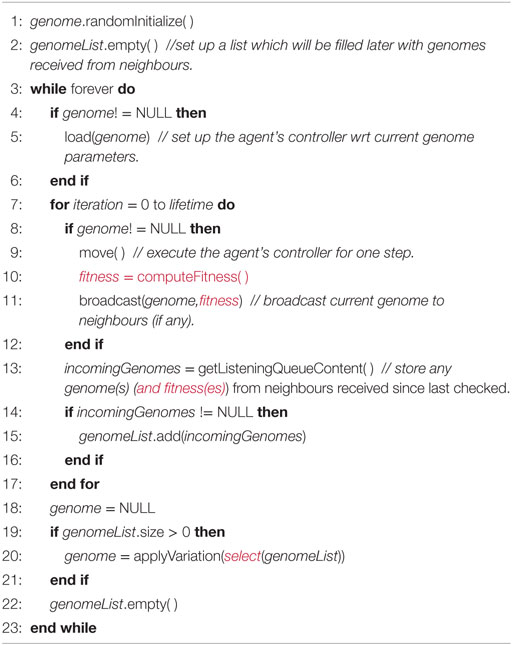
\includegraphics[width=0.5\textwidth]{imgalg.jpg}
    \caption{Basic "vanilla" version of embodied evolutionary robotics algorithm\cite{Rob1}.}
    \label{fig:eeal}
\end{wrapfigure}

\subsubsection{Evolutionary behaviours}

As a final experiment I've been proposed to team up with other two students in M1 Androide Parhams Shams and Tanguy Soto. As a part of a team I tested how the developed software could support an advanced robotics experiment.
Embodied evolutionary robotics describes a large area of evolutionary genetics algorythm applyed to robotics. Parhams Shams and Tanguy Soto implemented for their PAdroide final project an evolutionary algorithm for obstacle avoidance descripted in \cite{Rob1} and \cite{Rob2}, first in a non distribuited fashion so that the best behaviour was selected among the exemplar behaviour or fitting by a central system maximizing the fitness and broadcasting the genetic information, and a afterwards a distribuited version to be executed derectly on the Thymio robots in an areana. The fitness in this case is a function of a set of parameters like the distance or the number of times hitting an obstacle, the genetic infomations ore genome are a set of parameters for motors and sensors tuning the behaviour of the robots, the behaviour associated to an higher fitness is rewarded and carryed on as good genetic material but not before random mutation are added to the code, bad genetic material is discarded (natural selection). There are many variants for fitting functions and the selection of parameters and the ones implemented were proposed in \cite{Rob2}.

In Figure \ref{fig:eeal}\cite{Rob1} a basic "vanilla" version of a  embodied evuolutionary robotics algorithm is described in pseudocode. In the distributed version the genome is passed among neighbours, to experience its whereabouts a robot must be able to recognize other robots so that the instruction \textit{getListenintQueueCountet()} and \textit{broadcastGenomes(genome,fitness)} can be implemented correctly. 

The tag detection application served to sense neighbours and by binding tags to an ip address the robots could communicate and therefore share genetic information based on their proximity.

\subsection{Limits}

Motion blur affects largely tag detection, blurred edges lead to poor edge localization and this affects the detection capacity of the Canny algorithm. This is particularly noticeable when point of view is moving, a problem that has been overlooked when testing the system. In particular contigous edges are not detected by the Canny algorithm as shown in Figure \ref{fig:blur1} the contours of the tag are completely lost. An idea to cope with this effect could be to use a multiresolution system, as shown by preliminary tests. With a nearest interpolation and no spectral filtering jagged contours appears due to aliasing in a zone where previously no edge was detected. This is not a problem as long as contours are contiguous (Figure \ref{fig:blur2}) a tag can still be detected.

\begin{figure}[H]
    \centering
    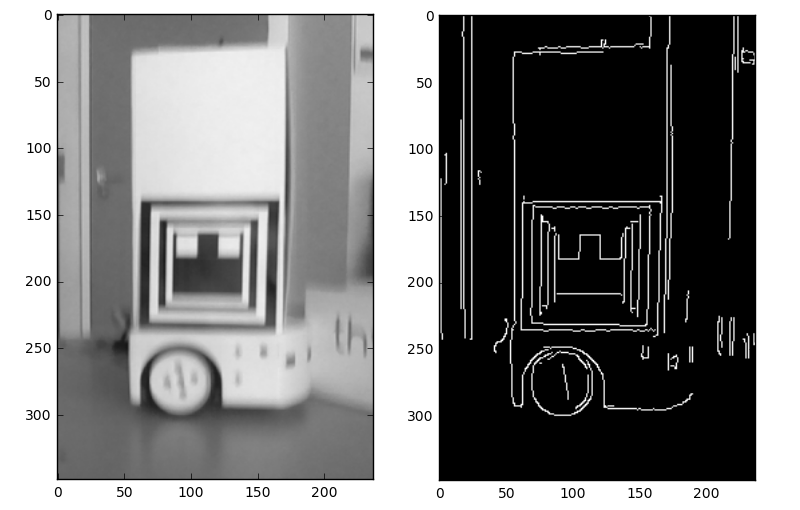
\includegraphics[width=0.7\textwidth]{BlurEdges.png}
    \caption{left: image affected by motion blur, right: Canny algorithm results applied on a motion blur affected image.}
    \label{fig:blur1}
     \centering
    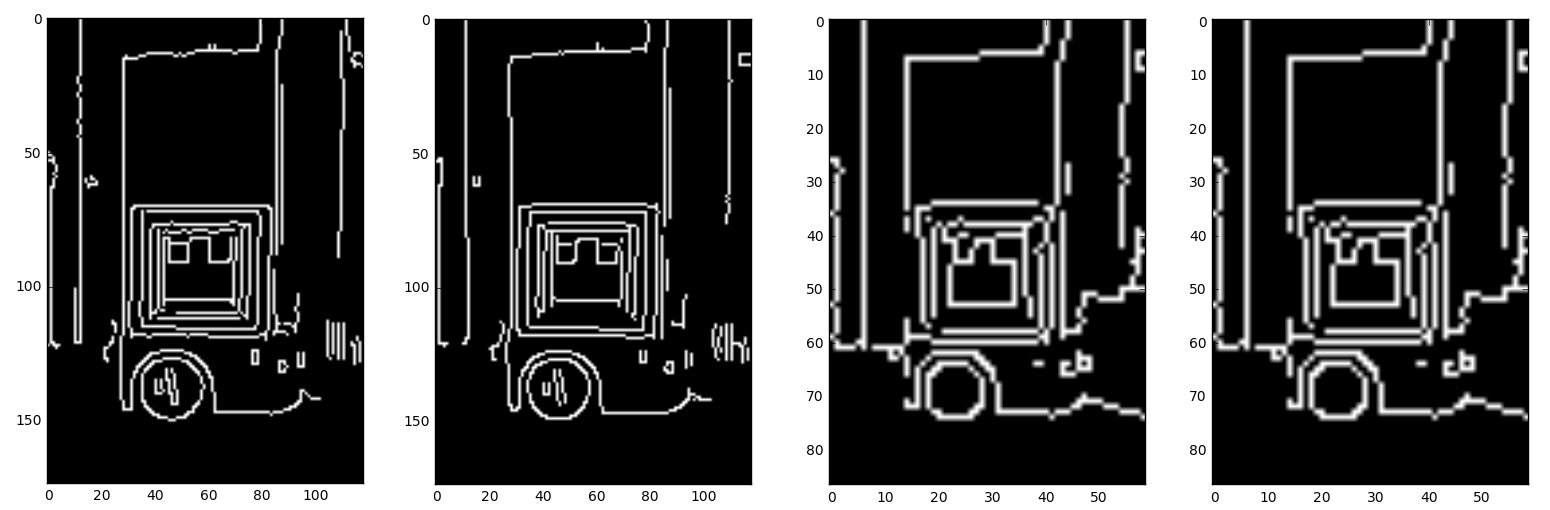
\includegraphics[width=1.0\textwidth]{BlurEdges_N2_L2_N4_L4.png}
    \caption{from left to right: half size Neareset interpolation, half size Linear interpolation, quarter size Nearest interpolation, quarter size Linear interpolation.}
    \label{fig:blur2}
\end{figure}

\section{Discussion}

Motion blur is currently the biggest obstacle that this implementation is facing. A complicated solution could be to deconvolve the motion blur with a known a priori point spread function PSF, but it is an expensive procedure and it may not work for all tags as they may be affected by different "amounts" of blur, so a single PSF is not meaningfull enough, a simpler solution could be binarizationm thresholding, this method will eventually find edges even in presence of poor localization, the downside of such method is that finding the optimal threshold is not a simple task. It has been envisioned a solution which involves getting the threshold by applying k-means for luminance quantization on the current image histogram and using the quatization values as thresholds similarly to the \textit{Otsu} method but with less parameters and with multiple thresholds. Something similar has been tried in early stages of the implementation but subsequently abandoned because of poor performances. Another possibility is to use a multiresolution system, motion blur affects the localization of edges but when definition is reduced and the image subsampled with nearest interpolation, delocalization of edges decrease, the motion detection analysis is also easier as it would need fewer levels. A qualitative test in this direction has been run upon suggestion of the advisor teacher Nicolas Bredeche and it looked promising (Figure \ref{fig:blur2}). Still another possibility is to use machine learning to fill in when detection is interrupted because of motion blur, another interesting solution would be to use "active tags" or led signals, this kind of tags would be easily detectable but this simplification comes with an increase in the cost of the robots.

\begin{thebibliography}{9}

\bibitem{Canny}J. Canny, "A Computational Approach to Edge Detection," vol. PAMI-8, no. 6, pp. 679-698, Nov. 1986.

\bibitem{LK}JJ.R. Bergen, P. Anandan, K. J. Hanna, R. Hingorani, "Hierarchical model-based motion estimation", Computer Vision - ECCV'92 pp. 237-252, May 1992.

\bibitem{QR}M. Hara, M. Watabe, T. Nojiri, T. Nagaya, Y. Uchiyama, "Optically readable twodimensional code and method and apparatus using the same" US 5 726 435, 10 mar 1998.

\bibitem{Performance}F. Yin, D. Makris, S. Velastin and Digital Imaging Research Centre, Kingston University
London, UK "Performance Evaluation of Object Tracking Algorithms" Computer Vision – ACCV 2006, pp. 151–161, Jan. 2006.

\bibitem{Rob1} N. Bredeche, E. Haasdijk, A. E. Eiben, On-Line, "On-Board Evolution of Robot Controllers", in Artifical Evolution: 9th International Conference, Evolution Artificielle, EA, 2009, Strasbourg, France, pp. 110-121, Oct 2009.

\bibitem{Rob2}J.M. Montanier, S. Carrignon, N. Bredeche "Behavioral specialization in embodied evolutionary robotics: Why so Difficult?" Front. Robot. AI vol.3 art 38, Jul 2016.

\bibitem{OpenCV}OpenCV Computer Vision Library. [Online]. Accessible: http://opencv.org/ [Accessed:23-May-2017].

\end{thebibliography}


\end{document}
